\documentclass{standalone}
\usepackage{tikz}
\usetikzlibrary{patterns, positioning}
\usepackage[sfdefault]{ClearSans} %% option 'sfdefault' activates Clear Sans as the default text font
\usepackage[T1]{fontenc}

\begin{document}
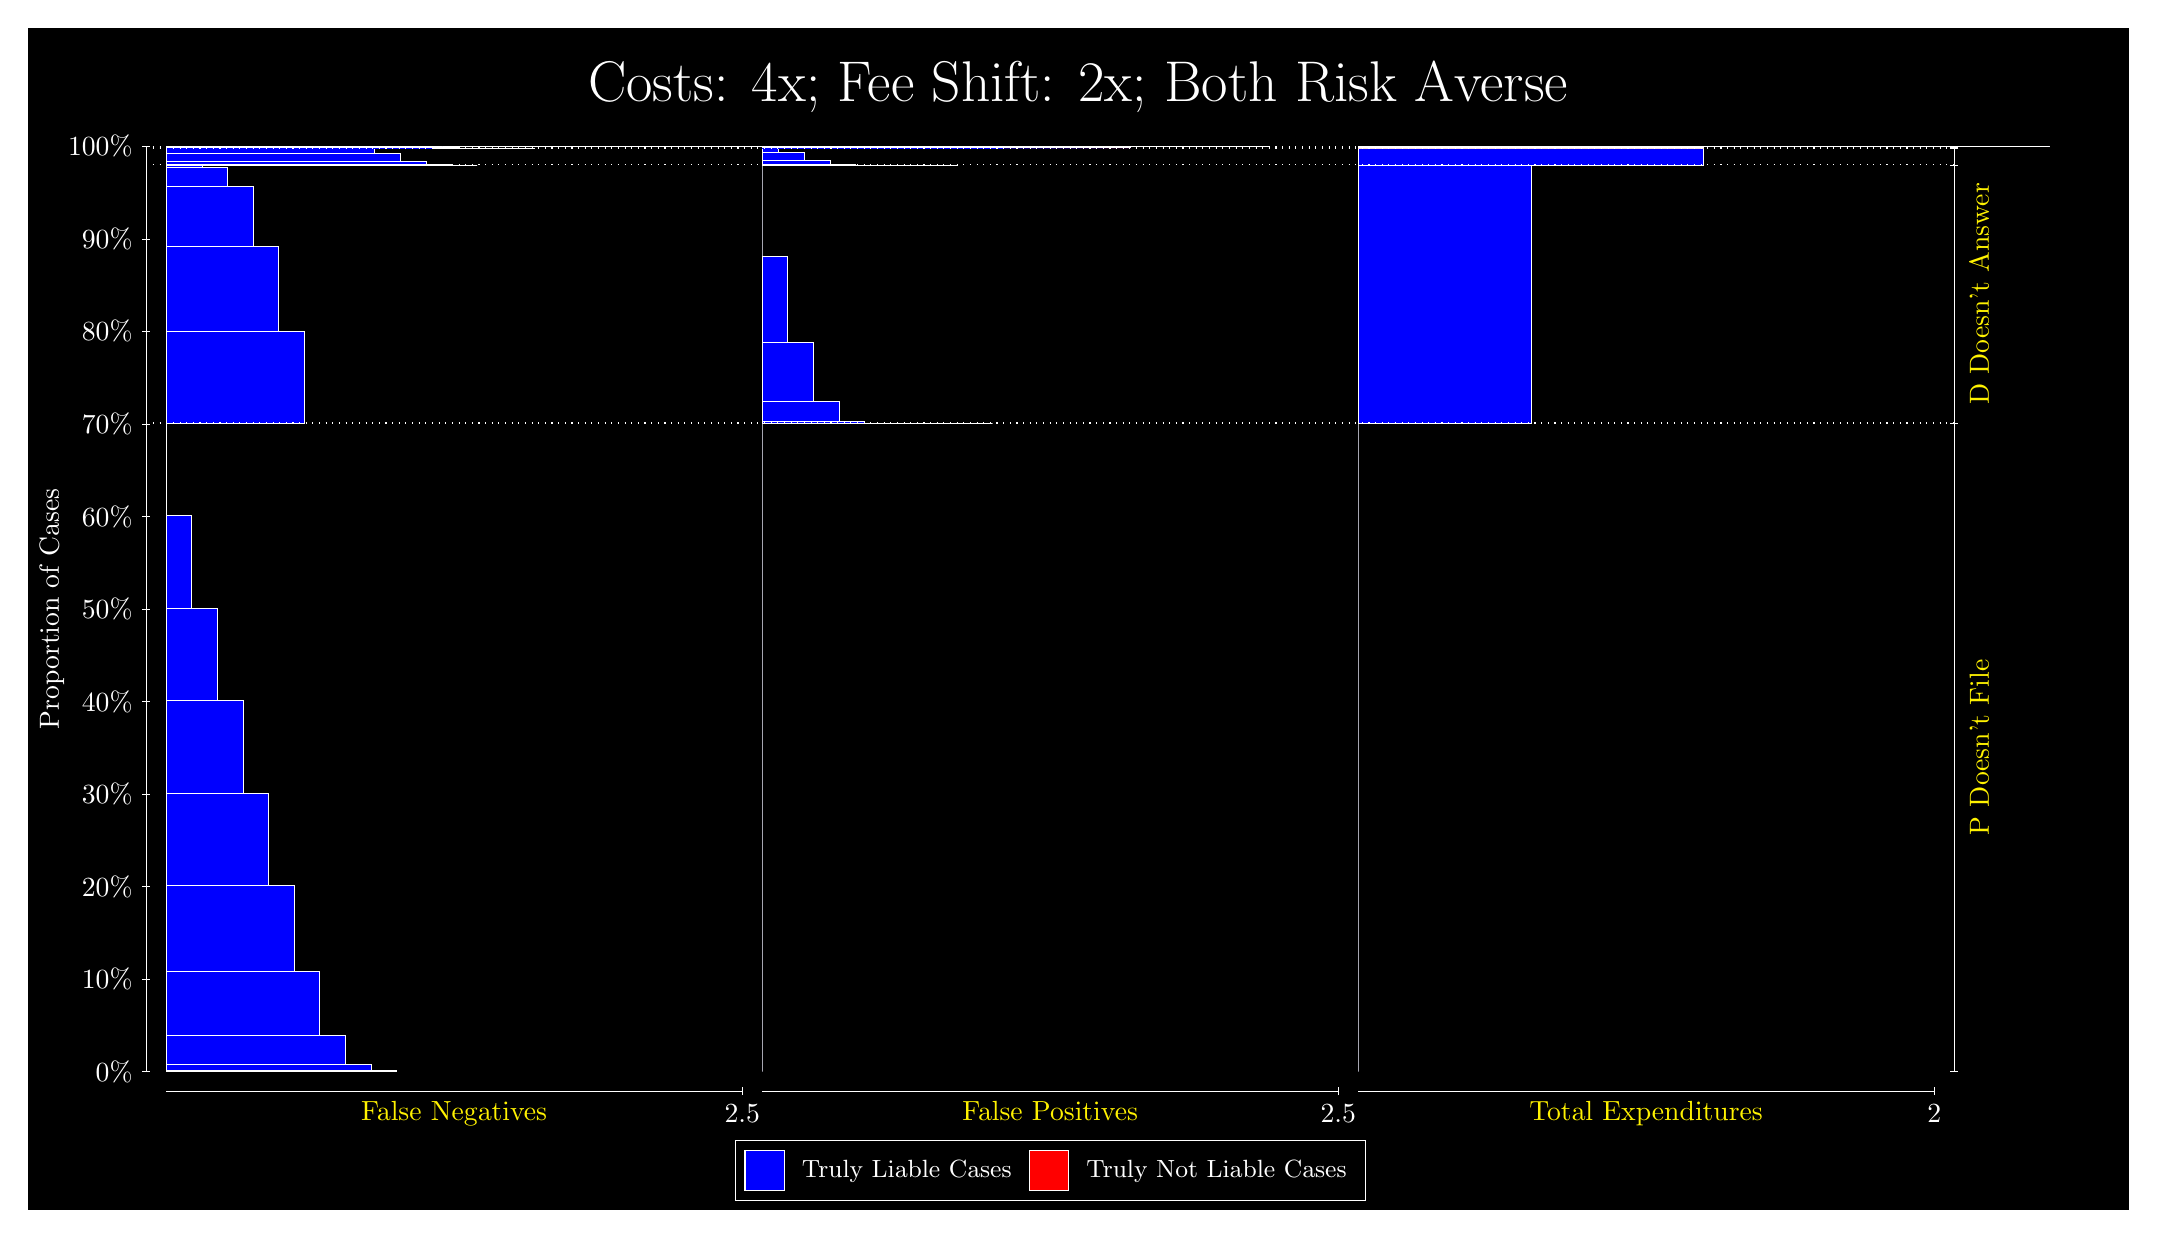
\begin{tikzpicture}
\draw[fill=black] (0,0) rectangle (26.667,15);
\draw[text=white] (0,13.5) rectangle (26.667,15) node[midway] {\huge Costs: 4x; Fee Shift: 2x; Both Risk Averse};
\draw[white, very thin] (1.5,1.75) -- (1.5,13.5);
\node[rotate=90, text=white, anchor=center] at (0.3, 7.625) {Proportion of Cases};
\draw[white, very thin] (1.45,1.75) -- (1.55,1.75);
\node[text=white, anchor=east] at (1.45, 1.75) {0\%};
\draw[white, very thin] (1.45,2.925) -- (1.55,2.925);
\node[text=white, anchor=east] at (1.45, 2.925) {10\%};
\draw[white, very thin] (1.45,4.1) -- (1.55,4.1);
\node[text=white, anchor=east] at (1.45, 4.1) {20\%};
\draw[white, very thin] (1.45,5.275) -- (1.55,5.275);
\node[text=white, anchor=east] at (1.45, 5.275) {30\%};
\draw[white, very thin] (1.45,6.45) -- (1.55,6.45);
\node[text=white, anchor=east] at (1.45, 6.45) {40\%};
\draw[white, very thin] (1.45,7.625) -- (1.55,7.625);
\node[text=white, anchor=east] at (1.45, 7.625) {50\%};
\draw[white, very thin] (1.45,8.8) -- (1.55,8.8);
\node[text=white, anchor=east] at (1.45, 8.8) {60\%};
\draw[white, very thin] (1.45,9.975) -- (1.55,9.975);
\node[text=white, anchor=east] at (1.45, 9.975) {70\%};
\draw[white, very thin] (1.45,11.15) -- (1.55,11.15);
\node[text=white, anchor=east] at (1.45, 11.15) {80\%};
\draw[white, very thin] (1.45,12.325) -- (1.55,12.325);
\node[text=white, anchor=east] at (1.45, 12.325) {90\%};
\draw[white, very thin] (1.45,13.5) -- (1.55,13.5);
\node[text=white, anchor=east] at (1.45, 13.5) {100\%};

\draw[white, very thin] (24.457,1.75) -- (24.457,13.5);
\draw[white, very thin] (24.407,1.75) -- (24.507,1.75);
\node[anchor=west] at (24.407, 1.75) {};
\draw[white, very thin] (24.407,9.986) -- (24.507,9.986);
\node[anchor=west] at (24.407, 9.986) {};
\draw[white, very thin] (24.407,13.265) -- (24.507,13.265);
\node[anchor=west] at (24.407, 13.265) {};
\draw[white, very thin] (24.407,13.477) -- (24.507,13.477);
\node[anchor=west] at (24.407, 13.477) {};
\draw[white, very thin] (24.407,13.484) -- (24.507,13.484);
\node[anchor=west] at (24.407, 13.484) {};
\draw[white, very thin] (24.407,13.5) -- (24.507,13.5);
\node[anchor=west] at (24.407, 13.5) {};
\draw[white, very thin] (24.407,13.5) -- (24.507,13.5);
\node[anchor=west] at (24.407, 13.5) {};

\draw[white, very thin, fill=blue] (1.75,1.75) rectangle (4.6775,1.7606);
\draw[white, very thin, fill=blue] (1.75,1.7606) rectangle (4.3523,1.8447);
\draw[white, very thin, fill=blue] (1.75,1.8447) rectangle (4.027,2.2095);
\draw[white, very thin, fill=blue] (1.75,2.2095) rectangle (3.7017,3.0221);
\draw[white, very thin, fill=blue] (1.75,3.0221) rectangle (3.3764,4.1186);
\draw[white, very thin, fill=blue] (1.75,4.1186) rectangle (3.0511,5.2863);
\draw[white, very thin, fill=blue] (1.75,5.2863) rectangle (2.7258,6.4611);
\draw[white, very thin, fill=blue] (1.75,6.4611) rectangle (2.4006,7.636);
\draw[white, very thin, fill=blue] (1.75,7.636) rectangle (2.0753,8.8111);
\draw[white, very thin, fill=red] (1.75,8.8111) rectangle (1.75,8.8111);
\draw[white, very thin, fill=blue] (1.75,8.8111) rectangle (1.75,9.986);
\draw[white, very thin, fill=blue] (1.75,9.986) rectangle (3.5065,11.15);
\draw[white, very thin, fill=blue] (1.75,11.15) rectangle (3.1812,12.234);
\draw[white, very thin, fill=blue] (1.75,12.234) rectangle (2.856,12.989);
\draw[white, very thin, fill=blue] (1.75,12.989) rectangle (2.5307,13.24);
\draw[white, very thin, fill=blue] (1.75,13.24) rectangle (2.2054,13.264);
\draw[white, very thin, fill=blue] (1.75,13.264) rectangle (1.8801,13.265);
\draw[white, very thin, fill=red] (1.75,13.265) rectangle (1.75,13.265);
\draw[white, very thin, fill=blue] (1.75,13.265) rectangle (1.75,13.265);
\draw[white, very thin, fill=blue] (1.75,13.265) rectangle (5.7022,13.265);
\draw[white, very thin, fill=blue] (1.75,13.265) rectangle (5.3769,13.269);
\draw[white, very thin, fill=blue] (1.75,13.269) rectangle (5.0516,13.313);
\draw[white, very thin, fill=blue] (1.75,13.313) rectangle (4.7263,13.417);
\draw[white, very thin, fill=blue] (1.75,13.417) rectangle (4.4011,13.47);
\draw[white, very thin, fill=blue] (1.75,13.47) rectangle (4.0758,13.476);
\draw[white, very thin, fill=blue] (1.75,13.476) rectangle (3.7505,13.477);
\draw[white, very thin, fill=blue] (1.75,13.477) rectangle (3.4252,13.477);
\draw[white, very thin, fill=blue] (1.75,13.477) rectangle (3.0999,13.477);
\draw[white, very thin, fill=blue] (1.75,13.477) rectangle (2.7746,13.477);
\draw[white, very thin, fill=red] (1.75,13.477) rectangle (1.75,13.477);
\draw[white, very thin, fill=blue] (1.75,13.477) rectangle (6.4341,13.477);
\draw[white, very thin, fill=blue] (1.75,13.477) rectangle (6.1088,13.477);
\draw[white, very thin, fill=blue] (1.75,13.477) rectangle (5.7835,13.48);
\draw[white, very thin, fill=blue] (1.75,13.48) rectangle (5.4582,13.483);
\draw[white, very thin, fill=blue] (1.75,13.483) rectangle (5.1329,13.484);
\draw[white, very thin, fill=blue] (1.75,13.484) rectangle (4.8077,13.484);
\draw[white, very thin, fill=blue] (1.75,13.484) rectangle (4.4824,13.484);
\draw[white, very thin, fill=blue] (1.75,13.484) rectangle (4.1571,13.484);
\draw[white, very thin, fill=blue] (1.75,13.484) rectangle (3.8318,13.484);
\draw[white, very thin, fill=blue] (1.75,13.484) rectangle (3.5065,13.484);
\draw[white, very thin, fill=red] (1.75,13.484) rectangle (1.75,13.484);
\draw[white, very thin, fill=blue] (1.75,13.484) rectangle (3.5065,13.484);
\draw[white, very thin, fill=blue] (1.75,13.484) rectangle (3.1812,13.487);
\draw[white, very thin, fill=blue] (1.75,13.487) rectangle (2.856,13.494);
\draw[white, very thin, fill=blue] (1.75,13.494) rectangle (2.5307,13.499);
\draw[white, very thin, fill=blue] (1.75,13.499) rectangle (2.2054,13.5);
\draw[white, very thin, fill=blue] (1.75,13.5) rectangle (1.8801,13.5);
\draw[white, very thin, fill=red] (1.75,13.5) rectangle (1.75,13.5);
\draw[white, very thin, fill=blue] (1.75,13.5) rectangle (1.75,13.5);
\draw[white, very thin, fill=blue] (1.75,13.5) rectangle (15.217,13.5);
\draw[white, very thin, fill=blue] (1.75,13.5) rectangle (14.891,13.5);
\draw[white, very thin, fill=blue] (1.75,13.5) rectangle (14.566,13.5);
\draw[white, very thin, fill=blue] (1.75,13.5) rectangle (14.241,13.5);
\draw[white, very thin, fill=blue] (1.75,13.5) rectangle (14.241,13.5);
\draw[white, very thin, fill=blue] (1.75,13.5) rectangle (13.916,13.5);
\draw[white, very thin, fill=blue] (1.75,13.5) rectangle (13.59,13.5);
\draw[white, very thin, fill=blue] (1.75,13.5) rectangle (13.265,13.5);
\draw[white, very thin, fill=blue] (1.75,13.5) rectangle (13.265,13.5);
\draw[white, very thin, fill=blue] (1.75,13.5) rectangle (12.94,13.5);
\draw[white, very thin, fill=blue] (1.75,13.5) rectangle (12.614,13.5);
\draw[white, very thin, fill=blue] (1.75,13.5) rectangle (12.289,13.5);
\draw[white, very thin, fill=blue] (1.75,13.5) rectangle (11.964,13.5);
\draw[white, very thin, fill=blue] (1.75,13.5) rectangle (11.639,13.5);
\draw[white, very thin, fill=blue] (1.75,13.5) rectangle (7.2148,13.5);
\draw[white, very thin, fill=blue] (1.75,13.5) rectangle (6.8895,13.5);
\draw[white, very thin, fill=blue] (1.75,13.5) rectangle (6.5642,13.5);
\draw[white, very thin, fill=blue] (1.75,13.5) rectangle (6.2389,13.5);
\draw[white, very thin, fill=blue] (1.75,13.5) rectangle (5.9136,13.5);
\draw[white, very thin, fill=blue] (1.75,13.5) rectangle (5.9136,13.5);
\draw[white, very thin, fill=blue] (1.75,13.5) rectangle (5.5883,13.5);
\draw[white, very thin, fill=blue] (1.75,13.5) rectangle (5.5883,13.5);
\draw[white, very thin, fill=blue] (1.75,13.5) rectangle (5.2631,13.5);
\draw[white, very thin, fill=blue] (1.75,13.5) rectangle (4.9378,13.5);
\draw[white, very thin, fill=blue] (1.75,13.5) rectangle (4.9378,13.5);
\draw[white, very thin, fill=blue] (1.75,13.5) rectangle (4.6125,13.5);
\draw[white, very thin, fill=blue] (1.75,13.5) rectangle (4.6125,13.5);
\draw[white, very thin, fill=blue] (1.75,13.5) rectangle (4.6125,13.5);
\draw[white, very thin, fill=blue] (1.75,13.5) rectangle (4.2872,13.5);
\draw[white, very thin, fill=blue] (1.75,13.5) rectangle (4.2872,13.5);
\draw[white, very thin, fill=blue] (1.75,13.5) rectangle (3.9619,13.5);
\draw[white, very thin, fill=blue] (1.75,13.5) rectangle (3.6366,13.5);
\draw[white, very thin, fill=blue] (1.75,13.5) rectangle (3.3114,13.5);
\draw[white, very thin, fill=blue] (1.75,13.5) rectangle (3.3114,13.5);
\draw[white, very thin, fill=blue] (1.75,13.5) rectangle (2.9861,13.5);
\draw[white, very thin, fill=blue] (1.75,13.5) rectangle (2.9861,13.5);
\draw[white, very thin, fill=blue] (1.75,13.5) rectangle (2.6608,13.5);
\draw[white, very thin, fill=blue] (1.75,13.5) rectangle (2.6608,13.5);
\draw[white, very thin, fill=blue] (1.75,13.5) rectangle (2.3355,13.5);
\draw[white, very thin, fill=red] (1.75,13.5) rectangle (1.75,13.5);
\draw[white, very thin, fill=red] (9.3189,1.75) rectangle (9.3189,1.75);
\draw[white, very thin, fill=blue] (9.3189,1.75) rectangle (9.3189,9.986);
\draw[white, very thin, fill=red] (9.3189,9.986) rectangle (12.246,9.986);
\draw[white, very thin, fill=blue] (9.3189,9.986) rectangle (12.246,9.986);
\draw[white, very thin, fill=blue] (9.3189,9.986) rectangle (11.921,9.986);
\draw[white, very thin, fill=blue] (9.3189,9.986) rectangle (11.596,9.986);
\draw[white, very thin, fill=blue] (9.3189,9.986) rectangle (11.271,9.986);
\draw[white, very thin, fill=blue] (9.3189,9.986) rectangle (10.945,9.9865);
\draw[white, very thin, fill=blue] (9.3189,9.9865) rectangle (10.62,10.011);
\draw[white, very thin, fill=blue] (9.3189,10.011) rectangle (10.295,10.261);
\draw[white, very thin, fill=blue] (9.3189,10.261) rectangle (9.9694,11.017);
\draw[white, very thin, fill=blue] (9.3189,11.017) rectangle (9.6442,12.101);
\draw[white, very thin, fill=blue] (9.3189,12.101) rectangle (9.3189,13.265);
\draw[white, very thin, fill=red] (9.3189,13.265) rectangle (11.807,13.265);
\draw[white, very thin, fill=blue] (9.3189,13.265) rectangle (11.807,13.265);
\draw[white, very thin, fill=blue] (9.3189,13.265) rectangle (11.482,13.265);
\draw[white, very thin, fill=blue] (9.3189,13.265) rectangle (11.157,13.265);
\draw[white, very thin, fill=blue] (9.3189,13.265) rectangle (10.831,13.265);
\draw[white, very thin, fill=blue] (9.3189,13.265) rectangle (10.506,13.272);
\draw[white, very thin, fill=blue] (9.3189,13.272) rectangle (10.181,13.324);
\draw[white, very thin, fill=blue] (9.3189,13.324) rectangle (9.8556,13.428);
\draw[white, very thin, fill=blue] (9.3189,13.428) rectangle (9.5303,13.472);
\draw[white, very thin, fill=blue] (9.3189,13.472) rectangle (9.3189,13.477);
\draw[white, very thin, fill=red] (9.3189,13.477) rectangle (11.075,13.477);
\draw[white, very thin, fill=blue] (9.3189,13.477) rectangle (11.075,13.477);
\draw[white, very thin, fill=blue] (9.3189,13.477) rectangle (10.75,13.477);
\draw[white, very thin, fill=blue] (9.3189,13.477) rectangle (10.425,13.477);
\draw[white, very thin, fill=blue] (9.3189,13.477) rectangle (10.1,13.477);
\draw[white, very thin, fill=blue] (9.3189,13.477) rectangle (9.7743,13.477);
\draw[white, very thin, fill=blue] (9.3189,13.477) rectangle (9.449,13.478);
\draw[white, very thin, fill=blue] (9.3189,13.478) rectangle (9.3189,13.484);
\draw[white, very thin, fill=red] (9.3189,13.484) rectangle (14.003,13.484);
\draw[white, very thin, fill=blue] (9.3189,13.484) rectangle (14.003,13.484);
\draw[white, very thin, fill=blue] (9.3189,13.484) rectangle (13.678,13.484);
\draw[white, very thin, fill=blue] (9.3189,13.484) rectangle (13.352,13.484);
\draw[white, very thin, fill=blue] (9.3189,13.484) rectangle (13.027,13.484);
\draw[white, very thin, fill=blue] (9.3189,13.484) rectangle (12.702,13.484);
\draw[white, very thin, fill=blue] (9.3189,13.484) rectangle (12.377,13.485);
\draw[white, very thin, fill=blue] (9.3189,13.485) rectangle (12.051,13.49);
\draw[white, very thin, fill=blue] (9.3189,13.49) rectangle (11.726,13.497);
\draw[white, very thin, fill=blue] (9.3189,13.497) rectangle (11.401,13.499);
\draw[white, very thin, fill=blue] (9.3189,13.499) rectangle (11.075,13.5);
\draw[white, very thin, fill=red] (9.3189,13.5) rectangle (15.759,13.5);
\draw[white, very thin, fill=blue] (9.3189,13.5) rectangle (15.759,13.5);
\draw[white, very thin, fill=blue] (9.3189,13.5) rectangle (15.434,13.5);
\draw[white, very thin, fill=red] (9.3189,13.5) rectangle (15.434,13.5);
\draw[white, very thin, fill=blue] (9.3189,13.5) rectangle (15.434,13.5);
\draw[white, very thin, fill=red] (9.3189,13.5) rectangle (15.109,13.5);
\draw[white, very thin, fill=blue] (9.3189,13.5) rectangle (15.109,13.5);
\draw[white, very thin, fill=blue] (9.3189,13.5) rectangle (15.109,13.5);
\draw[white, very thin, fill=blue] (9.3189,13.5) rectangle (14.784,13.5);
\draw[white, very thin, fill=red] (9.3189,13.5) rectangle (14.784,13.5);
\draw[white, very thin, fill=blue] (9.3189,13.5) rectangle (14.784,13.5);
\draw[white, very thin, fill=blue] (9.3189,13.5) rectangle (14.784,13.5);
\draw[white, very thin, fill=blue] (9.3189,13.5) rectangle (14.458,13.5);
\draw[white, very thin, fill=red] (9.3189,13.5) rectangle (14.458,13.5);
\draw[white, very thin, fill=blue] (9.3189,13.5) rectangle (14.458,13.5);
\draw[white, very thin, fill=blue] (9.3189,13.5) rectangle (14.458,13.5);
\draw[white, very thin, fill=blue] (9.3189,13.5) rectangle (14.133,13.5);
\draw[white, very thin, fill=red] (9.3189,13.5) rectangle (14.133,13.5);
\draw[white, very thin, fill=blue] (9.3189,13.5) rectangle (14.133,13.5);
\draw[white, very thin, fill=blue] (9.3189,13.5) rectangle (14.133,13.5);
\draw[white, very thin, fill=blue] (9.3189,13.5) rectangle (13.808,13.5);
\draw[white, very thin, fill=blue] (9.3189,13.5) rectangle (13.808,13.5);
\draw[white, very thin, fill=red] (9.3189,13.5) rectangle (13.808,13.5);
\draw[white, very thin, fill=blue] (9.3189,13.5) rectangle (13.808,13.5);
\draw[white, very thin, fill=blue] (9.3189,13.5) rectangle (13.808,13.5);
\draw[white, very thin, fill=blue] (9.3189,13.5) rectangle (13.482,13.5);
\draw[white, very thin, fill=blue] (9.3189,13.5) rectangle (13.482,13.5);
\draw[white, very thin, fill=blue] (9.3189,13.5) rectangle (13.482,13.5);
\draw[white, very thin, fill=blue] (9.3189,13.5) rectangle (13.157,13.5);
\draw[white, very thin, fill=blue] (9.3189,13.5) rectangle (13.157,13.5);
\draw[white, very thin, fill=blue] (9.3189,13.5) rectangle (13.157,13.5);
\draw[white, very thin, fill=blue] (9.3189,13.5) rectangle (12.832,13.5);
\draw[white, very thin, fill=blue] (9.3189,13.5) rectangle (12.832,13.5);
\draw[white, very thin, fill=blue] (9.3189,13.5) rectangle (12.832,13.5);
\draw[white, very thin, fill=blue] (9.3189,13.5) rectangle (12.507,13.5);
\draw[white, very thin, fill=blue] (9.3189,13.5) rectangle (12.507,13.5);
\draw[white, very thin, fill=blue] (9.3189,13.5) rectangle (12.507,13.5);
\draw[white, very thin, fill=blue] (9.3189,13.5) rectangle (12.181,13.5);
\draw[white, very thin, fill=blue] (9.3189,13.5) rectangle (12.181,13.5);
\draw[white, very thin, fill=blue] (9.3189,13.5) rectangle (12.181,13.5);
\draw[white, very thin, fill=blue] (9.3189,13.5) rectangle (11.856,13.5);
\draw[white, very thin, fill=blue] (9.3189,13.5) rectangle (11.856,13.5);
\draw[white, very thin, fill=blue] (9.3189,13.5) rectangle (11.531,13.5);
\draw[white, very thin, fill=blue] (9.3189,13.5) rectangle (11.531,13.5);
\draw[white, very thin, fill=blue] (9.3189,13.5) rectangle (11.206,13.5);
\draw[white, very thin, fill=blue] (9.3189,13.5) rectangle (10.88,13.5);
\draw[white, very thin, fill=red] (9.3189,13.5) rectangle (9.3189,13.5);
\draw[white, very thin, fill=blue] (9.3189,13.5) rectangle (9.3189,13.5);
\draw[white, very thin, fill=red] (16.888,1.75) rectangle (16.888,1.75);
\draw[white, very thin, fill=blue] (16.888,1.75) rectangle (16.888,9.986);
\draw[white, very thin, fill=red] (16.888,9.986) rectangle (19.083,9.986);
\draw[white, very thin, fill=blue] (16.888,9.986) rectangle (19.083,13.265);
\draw[white, very thin, fill=red] (16.888,13.265) rectangle (21.279,13.265);
\draw[white, very thin, fill=blue] (16.888,13.265) rectangle (21.279,13.477);
\draw[white, very thin, fill=red] (16.888,13.477) rectangle (21.279,13.477);
\draw[white, very thin, fill=blue] (16.888,13.477) rectangle (21.279,13.484);
\draw[white, very thin, fill=red] (16.888,13.484) rectangle (21.279,13.484);
\draw[white, very thin, fill=blue] (16.888,13.484) rectangle (21.279,13.5);
\draw[white, very thin, fill=red] (16.888,13.5) rectangle (25.67,13.5);
\draw[white, very thin, fill=blue] (16.888,13.5) rectangle (25.67,13.5);
\draw[white, very thin, fill=red] (16.888,13.5) rectangle (25.67,13.5);
\draw[white, very thin, fill=blue] (16.888,13.5) rectangle (25.67,13.5);
\draw[white, very thin, fill=red] (16.888,13.5) rectangle (25.67,13.5);
\draw[white, very thin, fill=blue] (16.888,13.5) rectangle (25.67,13.5);
\draw[white, dotted] (1.5,9.986) -- (24.457,9.986);
\draw[white, dotted] (1.5,13.265) -- (24.457,13.265);
\draw[white, dotted] (1.5,13.477) -- (24.457,13.477);
\draw[white, dotted] (1.5,13.484) -- (24.457,13.484);
\draw[white, dotted] (1.5,13.5) -- (24.457,13.5);
\draw[white, very thin] (1.75,1.5) -- (9.0689,1.5);
\node[text=yellow, anchor=north] at (5.4094, 1.5) {False Negatives};
\draw[white, very thin] (9.0689,1.45) -- (9.0689,1.55);
\node[text=white, anchor=north] at (9.0689, 1.45) {2.5};

\draw[white, very thin] (9.3189,1.5) -- (16.638,1.5);
\node[text=yellow, anchor=north] at (12.978, 1.5) {False Positives};
\draw[white, very thin] (16.638,1.45) -- (16.638,1.55);
\node[text=white, anchor=north] at (16.638, 1.45) {2.5};

\draw[white, very thin] (16.888,1.5) -- (24.207,1.5);
\node[text=yellow, anchor=north] at (20.547, 1.5) {Total Expenditures};
\draw[white, very thin] (24.207,1.45) -- (24.207,1.55);
\node[text=white, anchor=north] at (24.207, 1.45) {2};

\node[text=yellow, centered, rotate=90] at (24.777, 5.868) {P Doesn't File};
\node[text=yellow, centered, rotate=90] at (24.777, 11.625) {D Doesn't Answer};





\draw (12.978300999999998,1.5) node[draw=none] (baseCoordinate) {};
\begin{scope}[align=center]
        \matrix[scale=0.5, draw=white, below=0.5cm of baseCoordinate, nodes={draw}, column sep=0.1cm]{
            \node[rectangle, draw, minimum width=0.5cm, minimum height=0.5cm, fill=blue] {}; &
            \node[draw=none, font=\small, text=white] (B) {Truly Liable Cases}; &
            \node[rectangle, draw, minimum width=0.5cm, minimum height=0.5cm, fill=red] {}; &
            \node[draw=none, font=\small, text=white] (B) {Truly Not Liable Cases}; \\
            };
\end{scope}

\end{tikzpicture}
\end{document}